\documentclass[notes,11pt, aspectratio=169]{beamer}

\usepackage{pgfpages}
% These slides also contain speaker notes. You can print just the slides,
% just the notes, or both, depending on the setting below. Comment out the want
% you want.
\setbeameroption{hide notes} % Only slide
%\setbeameroption{show only notes} % Only notes
%\setbeameroption{show notes on second screen=right} % Both

\usepackage{helvet}
\usepackage[default]{lato}
\usepackage{array}
\usepackage{tgbonum}

\usepackage{tikz}
\usepackage{verbatim}
\setbeamertemplate{note page}{\pagecolor{yellow!5}\insertnote}
\usetikzlibrary{positioning}
\usetikzlibrary{snakes}
\usetikzlibrary{calc}
\usetikzlibrary{arrows}
\usetikzlibrary{decorations.markings}
\usetikzlibrary{shapes.misc}
\usetikzlibrary{matrix,shapes,arrows,fit,tikzmark}
\usepackage{amsmath}
\usepackage{mathpazo}
\usepackage{hyperref}
\usepackage{lipsum}
\usepackage{multimedia}
\usepackage{graphicx}
\usepackage{multirow}
\usepackage{graphicx}
\usepackage{dcolumn}
\usepackage{bbm}
\newcolumntype{d}[0]{D{.}{.}{5}}

\usepackage{changepage}
\usepackage{appendixnumberbeamer}
\newcommand{\beginbackup}{
   \newcounter{framenumbervorappendix}
   \setcounter{framenumbervorappendix}{\value{framenumber}}
   \setbeamertemplate{footline}
   {
     \leavevmode%
     \hline
     box{%
       \begin{beamercolorbox}[wd=\paperwidth,ht=2.25ex,dp=1ex,right]{footlinecolor}%
%         \insertframenumber  \hspace*{2ex} 
       \end{beamercolorbox}}%
     \vskip0pt%
   }
 }
\newcommand{\backupend}{
   \addtocounter{framenumbervorappendix}{-\value{framenumber}}
   \addtocounter{framenumber}{\value{framenumbervorappendix}} 
}


\usepackage{graphicx}
\usepackage[space]{grffile}
\usepackage{booktabs}
\newcommand\independent{\protect\mathpalette{\protect\independenT}{\perp}}
\def\independenT#1#2{\mathrel{\rlap{$#1#2$}\mkern2mu{#1#2}}}
\DeclareMathOperator{\Supp}{Supp}

% These are my colors -- there are many like them, but these ones are mine.
\definecolor{blue}{RGB}{0,114,178}
\definecolor{red}{RGB}{213,94,0}
\definecolor{yellow}{RGB}{240,228,66}
\definecolor{green}{RGB}{0,158,115}

\hypersetup{
  colorlinks=false,
  linkbordercolor = {white},
  linkcolor = {blue}
}


%% I use a beige off white for my background
\definecolor{MyBackground}{RGB}{255,253,218}

%% Uncomment this if you want to change the background color to something else
%\setbeamercolor{background canvas}{bg=MyBackground}

%% Change the bg color to adjust your transition slide background color!
\newenvironment{transitionframe}{
  \setbeamercolor{background canvas}{bg=yellow}
  \begin{frame}}{
    \end{frame}
}

\setbeamercolor{frametitle}{fg=blue}
\setbeamercolor{title}{fg=black}
\setbeamertemplate{footline}[frame number]
\setbeamertemplate{navigation symbols}{} 
\setbeamertemplate{itemize items}{-}
\setbeamercolor{itemize item}{fg=blue}
\setbeamercolor{itemize subitem}{fg=blue}
\setbeamercolor{enumerate item}{fg=blue}
\setbeamercolor{enumerate subitem}{fg=blue}
\setbeamercolor{button}{bg=MyBackground,fg=blue,}



% If you like road maps, rather than having clutter at the top, have a roadmap show up at the end of each section 
% (and after your introduction)
% Uncomment this is if you want the roadmap!
% \AtBeginSection[]
% {
%    \begin{frame}
%        \frametitle{Roadmap of Talk}
%        \tableofcontents[currentsection]
%    \end{frame}
% }
\setbeamercolor{section in toc}{fg=blue}
\setbeamercolor{subsection in toc}{fg=red}
\setbeamersize{text margin left=1em,text margin right=1em} 

\newenvironment{wideitemize}{\itemize\addtolength{\itemsep}{10pt}}{\enditemize}

\usepackage{environ}
\NewEnviron{videoframe}[1]{
  \begin{frame}
    \vspace{-8pt}
    \begin{columns}[onlytextwidth, T] % align columns
      \begin{column}{.70\textwidth}
        \begin{minipage}[t][\textheight][t]
          {\dimexpr\textwidth}
          \vspace{8pt}
          \hspace{4pt} {\Large \sc \textcolor{blue}{#1}}
          \vspace{8pt}
          
          \BODY
        \end{minipage}
      \end{column}%
      \hfill%
      \begin{column}{.38\textwidth}
        \colorbox{green!20}{\begin{minipage}[t][1.2\textheight][t]
            {\dimexpr\textwidth}
            Face goes here
          \end{minipage}}
      \end{column}%
    \end{columns}
  \end{frame}
}

\title[]{\textcolor{blue}{Interference, Spillovers and Dynamics}}
\author[PGP]{}
\institute[FRBNY]{\small{Paul Goldsmith-Pinkham}}


\begin{document}

%%% TIKZ STUFF
\tikzset{   
        every picture/.style={remember picture,baseline},
        every node/.style={anchor=base,align=center,outer sep=1.5pt},
        every path/.style={thick},
        }
\newcommand\marktopleft[1]{%
    \tikz[overlay,remember picture] 
        \node (marker-#1-a) at (-.3em,.3em) {};%
}
\newcommand\markbottomright[2]{%
    \tikz[overlay,remember picture] 
        \node (marker-#1-b) at (0em,0em) {};%
}
\tikzstyle{every picture}+=[remember picture] 
\tikzstyle{mybox} =[draw=black, very thick, rectangle, inner sep=10pt, inner ysep=20pt]
\tikzstyle{fancytitle} =[draw=black,fill=red, text=white]
%%%% END TIKZ STUFF

% Title Slide
\begin{frame}
\maketitle

\end{frame}

\begin{frame}{Final day of Part 1}
\begin{columns}[T] % align columns
  \begin{column}{.75\textwidth}
   \begin{wideitemize}
   \item Our discussions on identification in the potential outcomes
     framework have had several simplifying assumptions, which we will
     relax today.
     \begin{itemize}
     \item Binary scalar treatment
     \item Single time period (e.g. one treatment within the person)
     \item SUTVA -- Stable Unit Treatment Value Assignment
     \end{itemize}
  \end{wideitemize}

\end{column}%
  \hfill%
  \begin{column}{.5\textwidth}
    \begin{center}
    \end{center}
  \end{column}
\end{columns}
\end{frame}

\begin{frame}{Extending PO into multi-valued treatments}
\begin{columns}[T] % align columns
  \begin{column}{.6\textwidth}
  \begin{wideitemize}
  \item For simplicities' sake, we have focused on binary treatments
    so far. What if it's not?
  \item Let's start with a discrete, multi-valued treatment to start:
    $D_{i} \in \{0,1, \ldots, d\}$. You can rescale, etc. How should
    we consider the effects from this treatment?
    \pause
  \item This is straightforward! And all we need is the strong
    ignorability condition (the second term of SI is slightly more
    convoluted but intuitive)
  \item What if we have covariates? Or if we do linear regression here?
  \end{wideitemize}

\end{column}%
  \hfill%
  \begin{column}{.4\textwidth}
    \footnotesize
    \only<2->{
      \begin{align*}
        \tau_{i}(d, d') &= Y_{i}(d) - Y_{i}(d')\\
        E(\tau_{i}(d, d')) &= E(Y_{i}(d) - Y_{i}(d'))\\
                        &= E(Y_{i} | D_{i} = d) - E(Y_{i} | D_{i} = d')
      \end{align*}}
  \end{column}
\end{columns}
\end{frame}




\begin{frame}{Extending PO into multi-valued treatments - covariates and regression}
\begin{columns}[T] % align columns
  \begin{column}{.7\textwidth}
  \begin{wideitemize}
  \item Recall that our different approaches impute counterfactuals.  If we run a regression of
    \begin{equation*}
      Y_{i} = \tau D_{i} + \gamma X_{i} + \epsilon_{i},
    \end{equation*}
    we're asserting two things:
    \begin{enumerate}
    \item A linear approximation to the conditional expectation
    \item A linear relationship between $Y_{i}$ and $D_{i}$!
    \end{enumerate}
    When might we do that?
    \vspace{-7pt}
  \item The choice of approximating the effect of $D$ on $Y$ with a particular functional form can come from many places:
    \begin{enumerate}
    \item Data limitations: a linear model will be more accurately estimated (subject to the caveat that the functional form is right!)
    \item External validity: You may want to consider values of $d$
      that are not in the treatment set
    \end{enumerate}
\end{wideitemize}    


\end{column}%
  \hfill%
  \begin{column}{.4\textwidth}
  \end{column}
\end{columns}
\end{frame}


\begin{frame}{Extending PO into multi-valued treatments - covariates and regression}
\begin{columns}[T] % align columns
  \begin{column}{.4\textwidth}
  \begin{wideitemize}
  \item<1-> Let's make this concrete. Consider the following simulated
    data, where the effect is linear (just simulated such that
    $E(\tau_{i}(d, d') = d'-d$). (strict ignorability holds)
  \item<2-> Imposing model helps \emph{a lot} compared to non-parametric form
    \begin{itemize}
    \item But what do we do once we start thinking about controls?
    \item But if we're wrong about the model?
    \end{itemize}
\end{wideitemize}    

\end{column}%
  \hfill%
  \begin{column}{.6\textwidth}
    \only<1>{    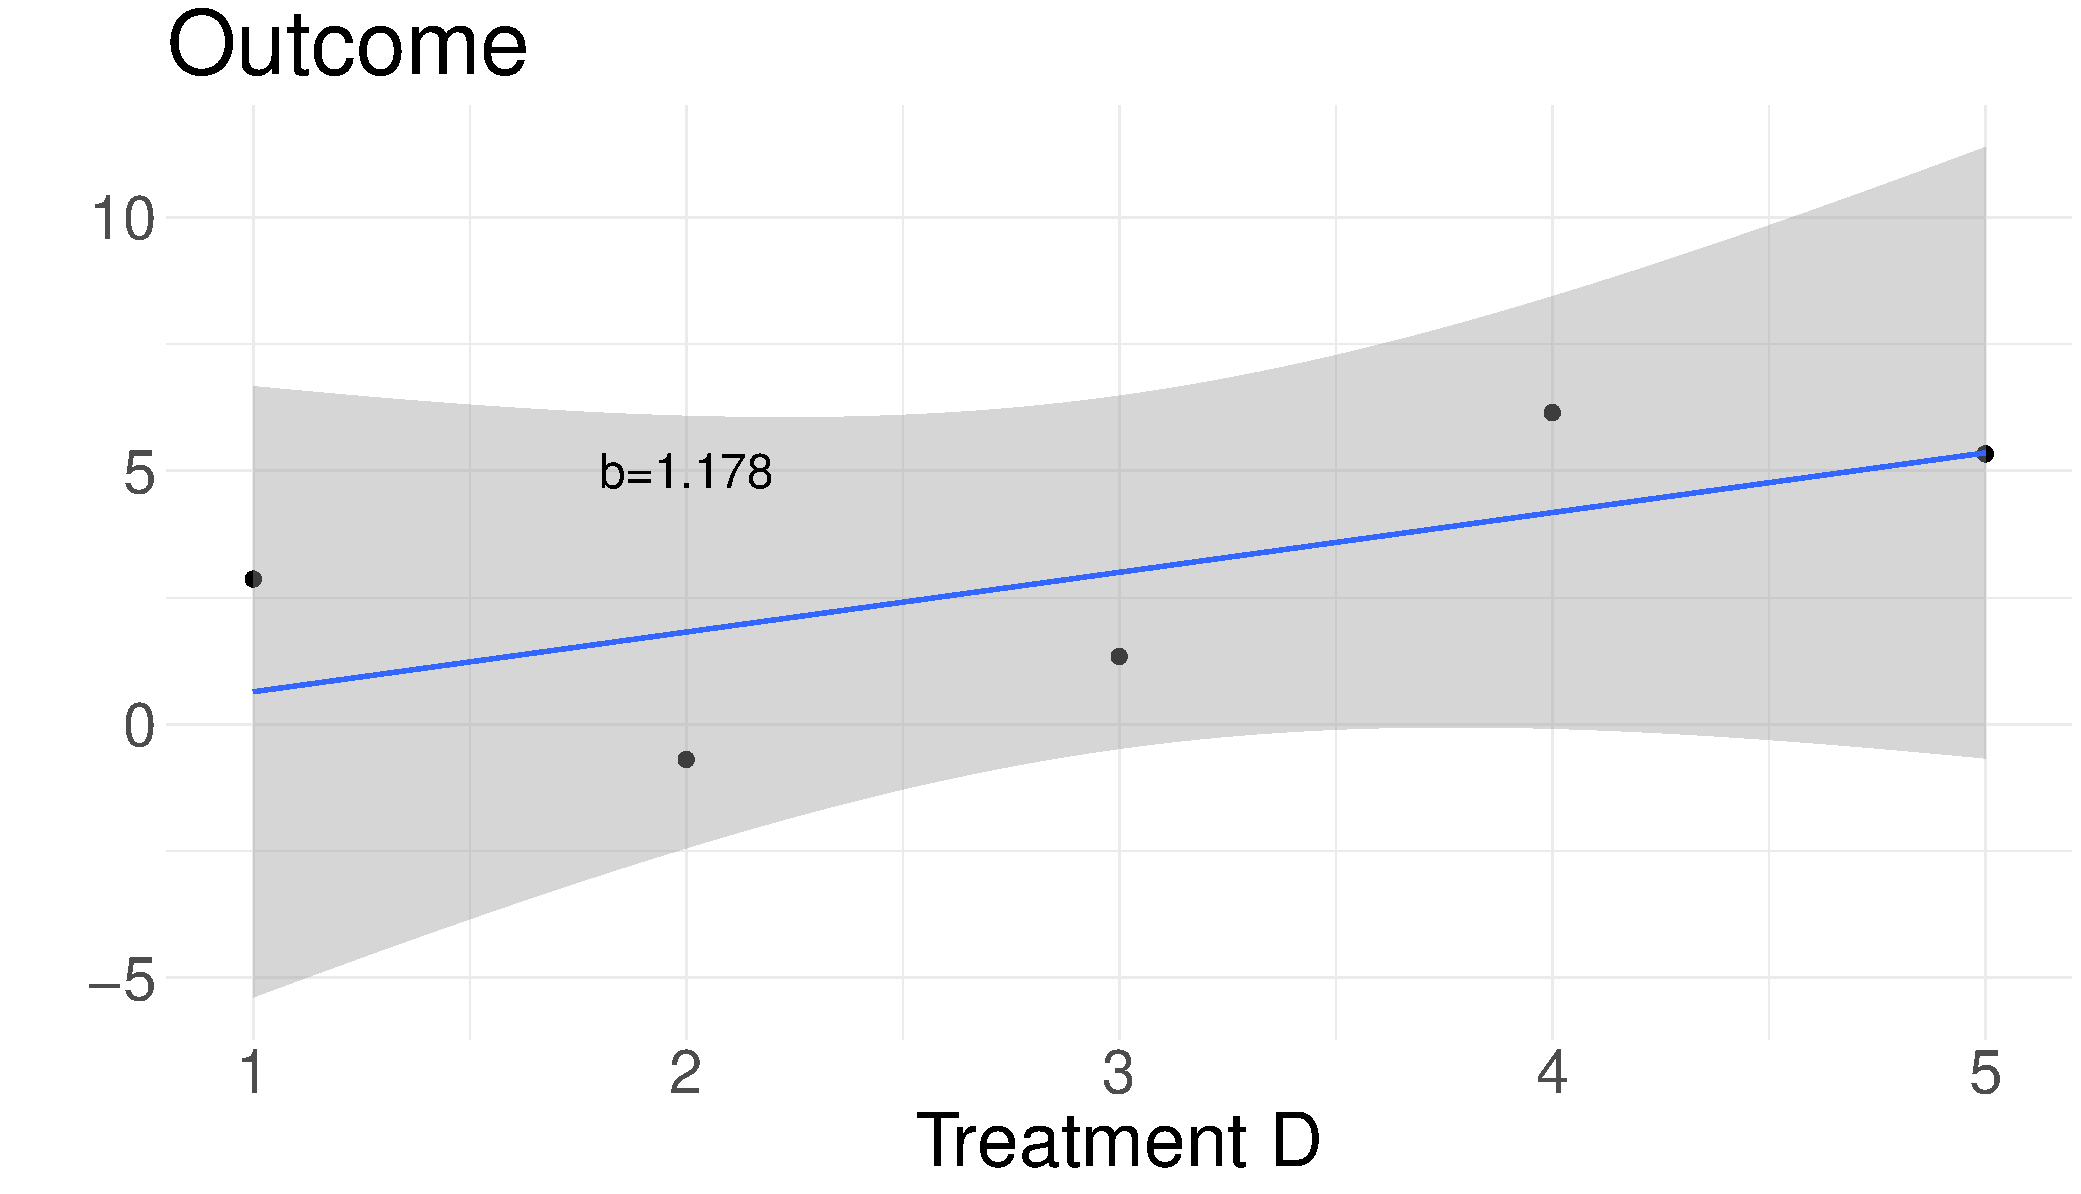
\includegraphics[width=\linewidth]{images/linear_multivalued.pdf}}
    \only<2>{    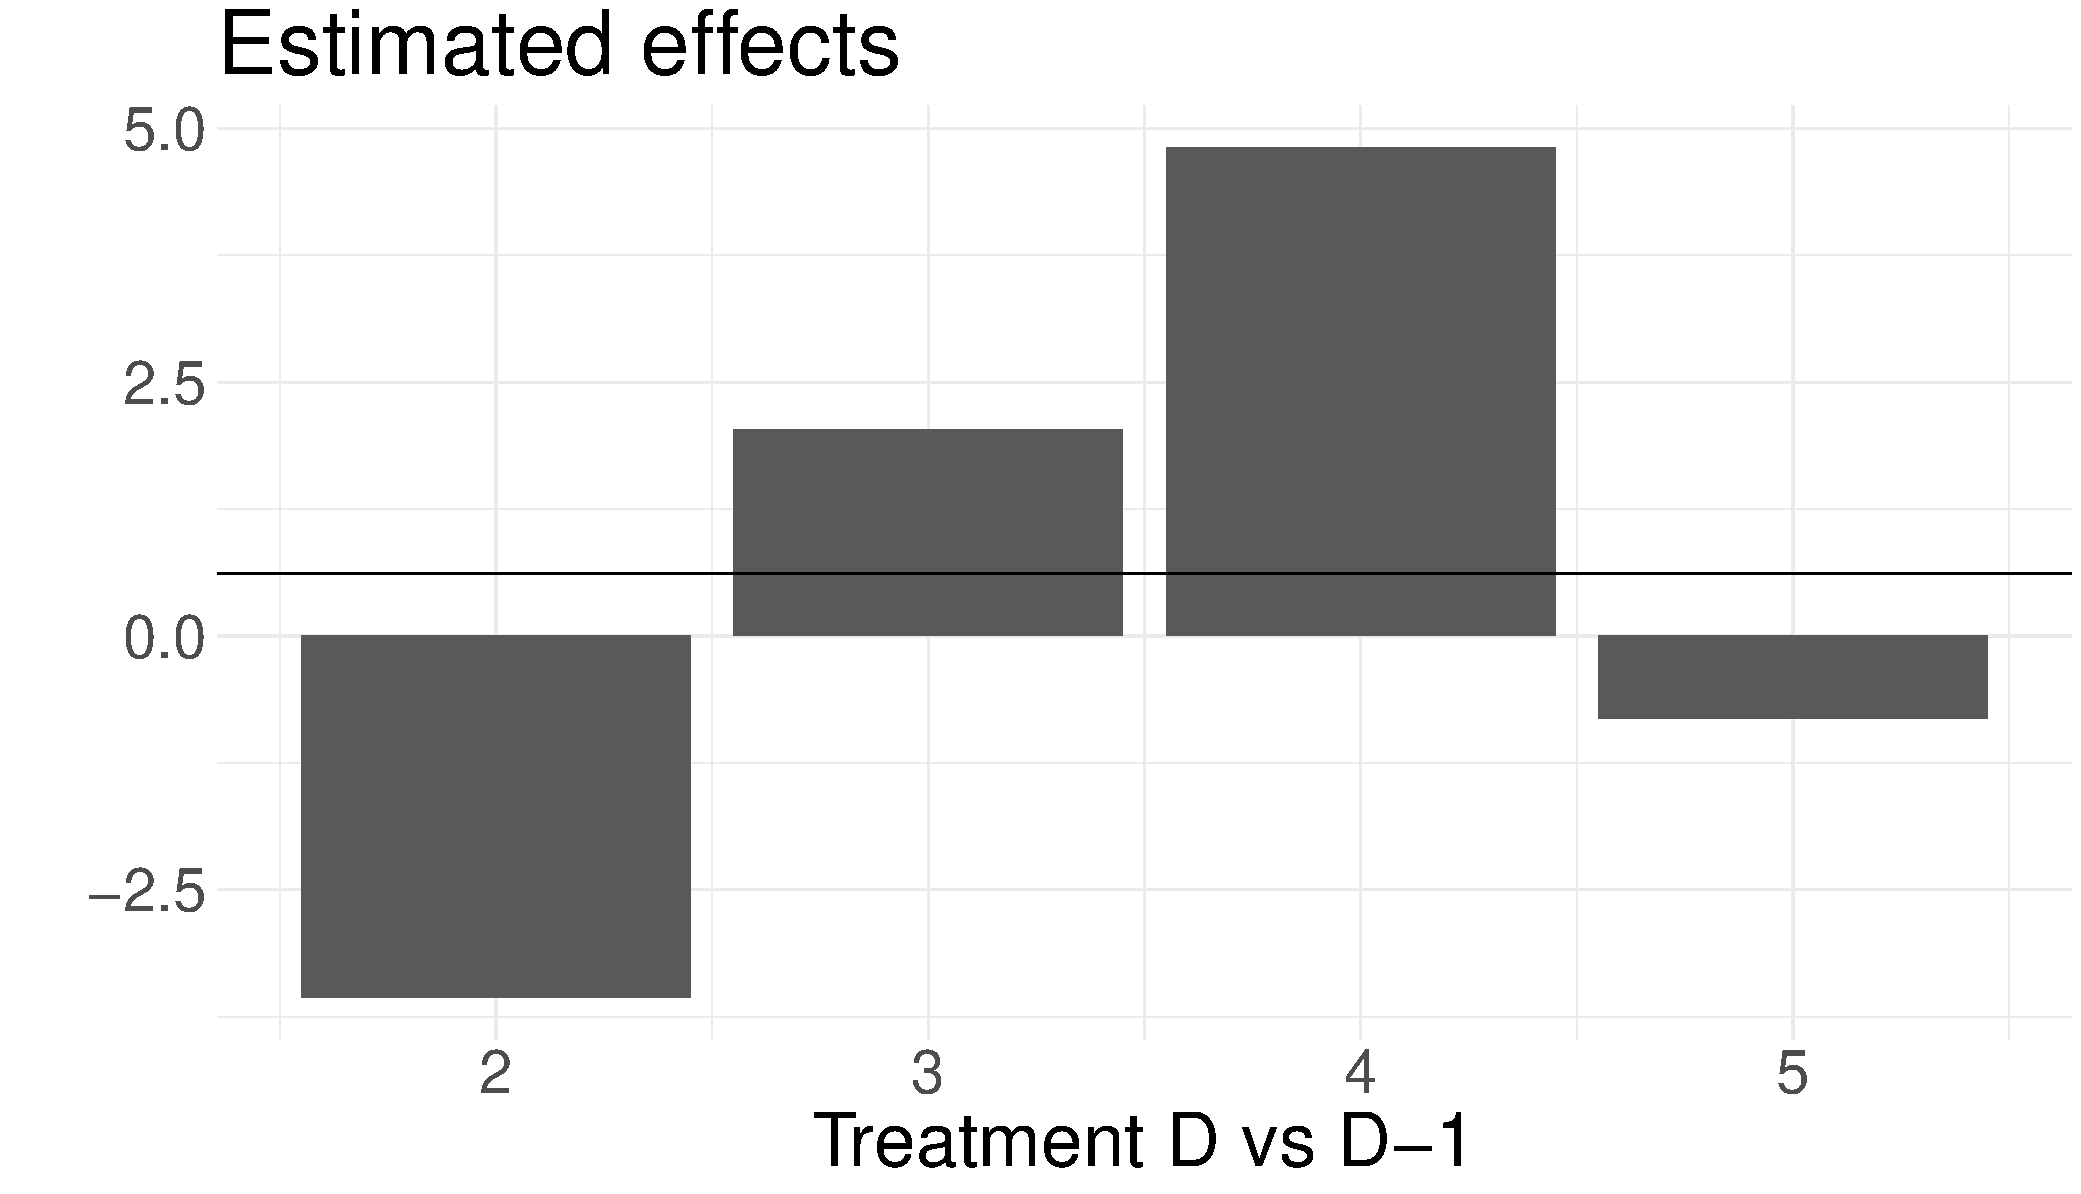
\includegraphics[width=\linewidth]{images/linear_multivalued2.pdf}}    
  \end{column}
\end{columns}
\end{frame}




\begin{frame}{Extending PO into multi-valued treatments}
\begin{columns}[T] % align columns
  \begin{column}{.75\textwidth}
    \begin{wideitemize}
    \item This is all a relatively familiar problem in econometrics
      \begin{itemize}
      \item Substantial structural work testing different parametric forms
      \item Non-parametric work dominates parametric work in terms of
        ``reducing assumptions'' but is extremely data hungry
      \item Once the dimension of any control variables is high,
        restrictions on the models will be necessary, especially with
        multivalued treatments
      \end{itemize}
    \item We'll discuss some of these \emph{estimation} issues later, but  key issue today is thinking about identification
      \begin{itemize}
      \item Non-parametric version was feasible because strong ignorability and SUTVA across individuals
      \end{itemize}
  \end{wideitemize}    

\end{column}%
  \hfill%
  \begin{column}{.5\textwidth}
  \end{column}
\end{columns}
\end{frame}



\begin{frame}{Extending PO into multi-valued treatments - multiple treatments}
\begin{columns}[T] % align columns
  \begin{column}{.6\textwidth}
    \begin{wideitemize}
    \item Important note so far: $D$ was an \emph{ordered} multivalued
      treatment.
    \item What if now, $\mathbf{D}_{i} \in \{0,1\}^{2}$ -- two binary
      treatments (you could encode this as a multivalued treatment,
      and then the ordering is likely meaningless)
    \item How should we model this? The most natural way is
      $Y_{i}(D_{i1}, D_{i2})$ -- each treatment flexibly affecting the
      outcome
\end{wideitemize}    

\end{column}%
  \hfill%
  \begin{column}{.4\textwidth}
    \begin{tabular}{c|rr}
      $ Y_{i}(\mathbf{D_{i}})$ & $D_{1i} = 0$ & $D_{1i} = 1$\\
      \midrule
      $D_{2i} = 0$ & $Y_{i}(0,0)$ & $Y_{i}(1,0)$\\
      $D_{2i} = 1$ & $Y_{i}(0,1)$ & $Y_{i}(1,1)$\\
    \end{tabular}
    
    \begin{itemize}
    \item  What is our estimand now?
    \item Let $\tau(\mathbf{d}, \mathbf{d}') = E(Y_{i}(d_{1},d_{2}) - Y_{i}(d'_{1},d'_{2})) $
    \item So many choices! What is the most relevant estimand? What
      exploits the most amount of data?
    \item Most important: \emph{what is identifiable}?
    \end{itemize}
  \end{column}
\end{columns}
\end{frame}



\begin{frame}{Extending PO into multi-valued treatments - multiple treatments}
\begin{columns}[T] % align columns
  \begin{column}{.6\textwidth}
    \begin{wideitemize}
    \item When there are multiple (unordered) treatments, it is
      important to have clarity on what your estimand is
    \item Consider a case where you have $K$ teachers that you can
      assign in a classroom
      \begin{itemize}
      \item What is the relevant treatment estimand?
      \item What would you want to report?
      \end{itemize}
      \pause 
    \item We will discuss in linear regression issues that can arise
      with these settings if you are not careful (see
      Goldsmith-Pinkham, Hull and Koles\'ar (2022) for a discussion)
\end{wideitemize}    

\end{column}%
  \hfill%
  \begin{column}{.4\textwidth}
  \end{column}
\end{columns}
\end{frame}



\begin{frame}{Intuition building with multi-valued treatments}
\begin{columns}[T] % align columns
  \begin{column}{.7\textwidth}
    \begin{wideitemize}
    \item What is an example of $\tau(\mathbf{d}, \mathbf{d}')$ that
      would not be identifiable, even if $\mathbf{d}$ is randomly
      assigned?
      \pause
    \item What if $D_{2i}$ is only given at times when $D_{1i}$ is given?
      \begin{itemize}
      \item Then, it's never possible to identify the effect relative
        to $Y_{i}(0,1)$
      \item What does that imply about our other potential estimands?
      \item E.g. if we just looked at the \emph{marginal} estimands,
        where we were estimating the effect of one treatment,
        $E(Y_{i}(1, D_{i2}) - Y_{i}(0, D_{i2}))$ -- this would
        integrate over joint distribution of treatments
      \end{itemize}
    \item In this example, $D_{2}$ is no longer conditionally
      ignorable -- the vector itself could be, but not individual components
    \item In most simple cases with multiple treatments, you'd
      randomize along multiple arms, and this problem is avoided
    \end{wideitemize}    

\end{column}%
  \hfill%
  \begin{column}{.3\textwidth}
    \begin{center}
      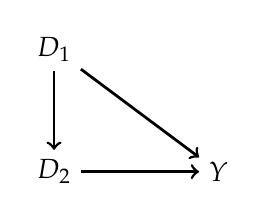
\begin{tikzpicture}
        % nodes %
        % \node[text centered] (z) {$Z$};
        \node[text centered] (t) {$D_{2}$};
        \node[right=1.5 of t, text centered] (y) {$Y$};
        \node[ above = 1 of t, text centered] (u) {$D_{1}$};

        % edges %
        % \draw[->, line width= 1] (z) --  (t);
        \draw [->, line width= 1] (t) -- (y);
        % \draw[->,red, line width= 1,dashed] (u) --node {X} (z);
        \draw[->,line width= 1] (u) --(t);
        \draw[->,line width= 1] (u) -- (y);
%\draw[->, red, line width=1,dashed] (z) to  [out=270,in=270, looseness=0.5] node{X} (y);
      \end{tikzpicture}
    \end{center}
  \end{column}
\end{columns}
\end{frame}


\begin{frame}{CONSORT diagram}
  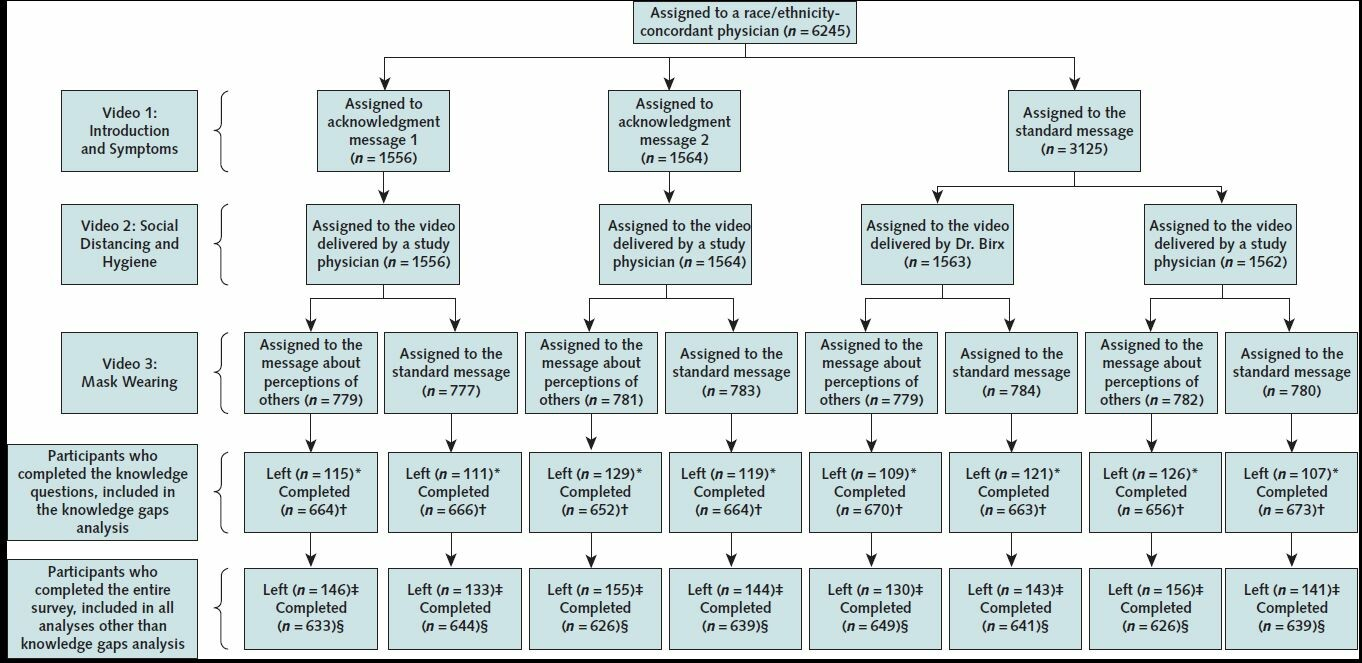
\includegraphics[width=\linewidth]{images/consort.jpeg}
\end{frame}

\begin{frame}{Now, the SUTVA hits the fan}
\begin{columns}[T] % align columns
  \begin{column}{.7\textwidth}
    \begin{wideitemize}
    \item In the discussion so far, the ``interference'' between
      treatments just comes from having multiple treatments to worry
      about
    \item What if treatments spill across units?
    \item Recall SUTVA: the potential outcomes of a unit do not vary
      with the treatment of other units
    \item When could this be violated?
      \begin{itemize}
      \item \emph{So many places}
      \end{itemize}
    \item Why does this create an issue? Recall our discussion regarding marginal estimands -- even with random assignment, our estimates of an effect will be contaminated by others' treatment status
    \end{wideitemize}    

\end{column}%
  \hfill%
  \begin{column}{.3\textwidth}
    \begin{center}
      \only<1>{
      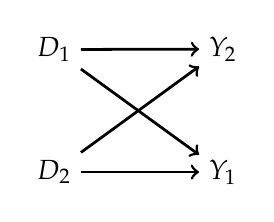
\begin{tikzpicture}
        % nodes %
        % \node[text centered] (z) {$Z$};
        \node[text centered] (t) {$D_{2}$};
        \node[right=1.5 of t, text centered] (y) {$Y_{1}$};
        \node[above=1 of y, text centered] (y2) {$Y_{2}$};        
        \node[ above = 1 of t, text centered] (u) {$D_{1}$};

        % edges %
        % \draw[->, line width= 1] (z) --  (t);
        \draw [->, line width= 1] (t) -- (y);
        \draw [->, line width= 1] (t) -- (y2);        
        % \draw[->,red, line width= 1,dashed] (u) --node {X} (z);
        \draw[->,line width= 1] (u) --(y2);        
        \draw[->,line width= 1] (u) -- (y);
%\draw[->, red, line width=1,dashed] (z) to  [out=270,in=270, looseness=0.5] node{X} (y);
      \end{tikzpicture}}
    \end{center}
  \end{column}
\end{columns}
\end{frame}


\begin{frame}{An overview of the types of issues caused by SUTVA not holding}
  \begin{columns}[T] % align columns
    \begin{column}{.7\textwidth}
      \begin{wideitemize}
      \item This type of problem is generally referred to as ``interference.''
        \begin{itemize}
        \item It is challenging in a number of ways -- for identification, estimation and inference
        \item Today we'll focus on identification
        \end{itemize}
      \item Want to touch on three versions of this problem:        
        \begin{enumerate}
        \item Social interactons and peer effects
        \item Spatial spillovers
        \item Economic interactions -- budget constraints, etc.
        \end{enumerate}
      \item All these problems are versions of violation of SUTVA
        \begin{itemize}
        \item With a clean, well-identified experiment, many of these
          settings still work
        \item However, to get the estimands we're interested in, we
          may have to substantially modify our traditional estimators or make strong assumptions
        \end{itemize}
      \end{wideitemize}
  \end{column}%
  \hfill%
  \begin{column}{.5\textwidth}
    \begin{center}
    \end{center}
  \end{column}
\end{columns}

\end{frame}


\begin{frame}{Networks}
\begin{columns}[T] % align columns
  \begin{column}{.5\textwidth}
    \begin{wideitemize}
    \item Historical context: Manski (1993)
      \begin{itemize}
      \item Paper focused on a linear-in-means structural equation
        \begin{align*}
          Y &= \underbrace{\beta E(Y|g)}_{\text{endogeneous}} + \underbrace{\gamma_{1} E(X|g)}_{\text{exogeneous}} + \gamma_{2} X\\
          &+ \underbrace{\gamma_{3} g}_{\text{contextual}} + u 
        \end{align*}
      \end{itemize}
    \item Peers were not well-defined but usually groups like
      classrooms, clubs, etc.
    \item This is a \emph{structural} model. RF:
      \begin{align*}
        Y &=  \gamma_{1}/(1-\beta) E(X|g) + (\gamma_{2}/(1-\beta)) X\\
          &+ (\gamma_{3}/(1-\beta)) g + \tilde{u} 
        \end{align*}

    \end{wideitemize}
  \end{column}%
  \hfill%
  \begin{column}{.5\textwidth}
    \begin{center}
      
\includegraphics[width=\linewidth]{images/manski0.png}\\
      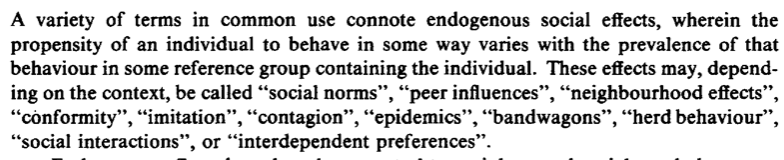
\includegraphics[width=\linewidth]{images/manski1.png}\\
      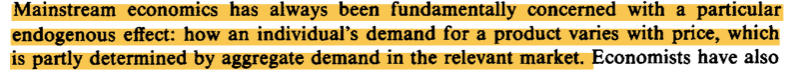
\includegraphics[width=\linewidth]{images/manski2.png}\\
      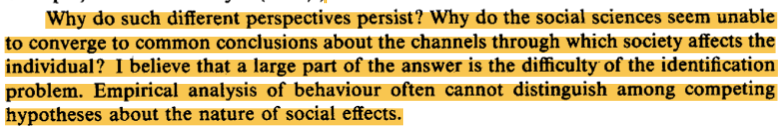
\includegraphics[width=\linewidth]{images/manski3.png}            
    \end{center}
  \end{column}
\end{columns}
\end{frame}

\begin{frame}{Large literature built off of this}
  \begin{wideitemize}
  \item Manski (1993) spawned a huge literature, a lot of which
    focused on the linear-in-means model.
    \begin{itemize}
    \item There's a literature that microfounds why you might use it
    \end{itemize}
  \item An inherent issue, in my view, is that many empirical papers
    jumped to this construction immediately. They did not have a
    structural interpretation in mind, but used this setting as a way
    to test for effects.
  \item An innovation in this space was to start using network data to define the group structure
    \begin{itemize}
    \item One key paper that moved to network version:  Bramoull\'e et al. (2009)
    \item Reframe Manski Linear-in-means model to
      \begin{align*}
        Y &= \beta AY  + \gamma_{1} AX + \gamma_{2}X + \epsilon_{i},\\
          &=   (I-\beta A)^{-1}\gamma_{1} AX + (I-\beta A)^{-1}\gamma_{2}X + (I-\beta A)^{-1}\epsilon_{i} 
      \end{align*}
      where $A$ is an $n \times n$ matrix of individuals'
      connections. Again, structural, but now richer interactions
    \end{itemize}
  \end{wideitemize}
\end{frame}

\begin{frame}{Design-based approach to peer effects}
  \begin{wideitemize}
  \item Taking the point of view of evaluation, or design-baesd
    inference, setting up the empirical model in this way is somewhat confusing
  \item Instead, useful to think about the general form of social
    interactions that are identified in a potential outcomes framework
  \item Given $n$ individuals, for person $i$, how much interference can we allow? What types?
    \begin{equation*}
      Y_{i}(D_{1}, D_{2}, \ldots, D_{n})
    \end{equation*}
    is far more extreme than
    \begin{equation*}
      Y_{i}(D_{i}, A\mathbf{D}_{n}).
    \end{equation*}
  \item This is a very active literature
  \end{wideitemize}
\end{frame}

\begin{frame}{Networks}
\begin{columns}[T] % align columns
  \begin{column}{.5\textwidth}
    \begin{wideitemize}
    \item There is no ``one solution'' in this setting
    \item Certain restrictions need to be made to identify some estimands
    \item Manski (2013) is a very nice discussion of this in a
      \emph{very} high-level way
      \begin{itemize}
      \item Warning: this paper can make you feel overwhelmed
      \item It is fine to make restrictive assumptions to identify effects!
      \end{itemize}
    \item Key point to identify in this literature -- are you
      attempting to estimate the \emph{spillover} effect, or are you
      attempting to identify individual ATE in the presence of
      spillovers?
    \end{wideitemize}
  \end{column}%
  \hfill%
  \begin{column}{.5\textwidth}
    \begin{center}
      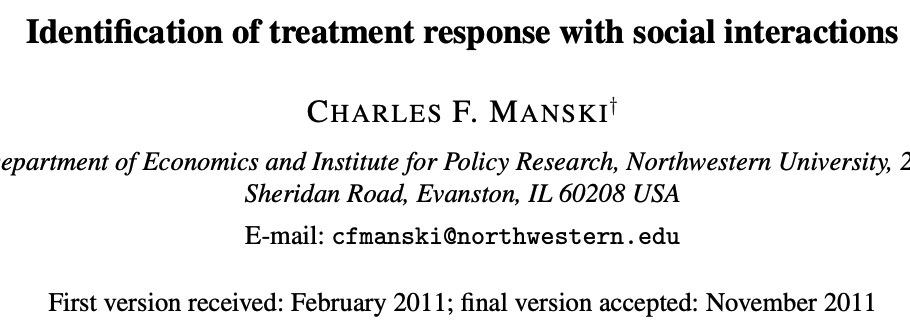
\includegraphics[width=\linewidth]{images/manski4b.png}\\
      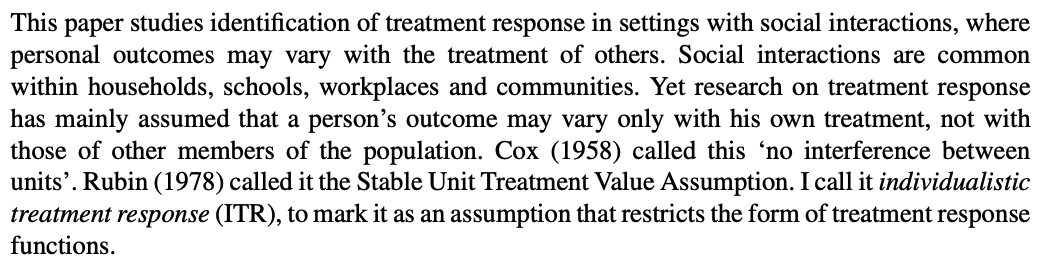
\includegraphics[width=\linewidth]{images/manski5.png}\\
      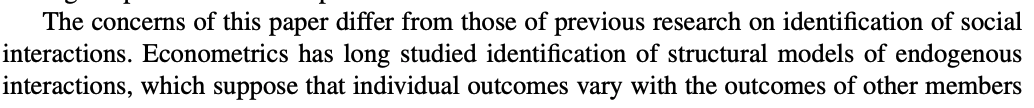
\includegraphics[width=\linewidth]{images/manski6.png}\\
            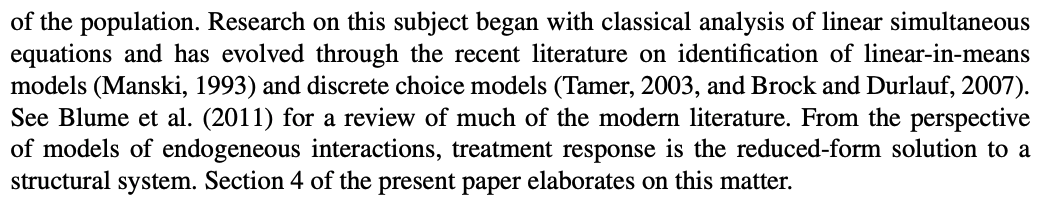
\includegraphics[width=\linewidth]{images/manski7.png}\\
    \end{center}
  \end{column}
\end{columns}
\end{frame}


\begin{frame}{Two papers in this space - Aronow and Samii (2017)}
    \begin{wideitemize}
    \item Aronow and Samii (2017) provide a framework for thinking
      about estimation and identification under general forms of
      interference
    \item A\&S use design-based inference, and consider the following
      generalized mapping.
      \begin{itemize}
      \item For any generalized vector of interventions,
        $\mathbf{D}_{n}$, there's an experimental design which assigns
        probabilities over this (this is familiar!)
      \item There is then an \emph{exposure} mapping
        $f(\mathbf{D}_{n}, \theta_{i})$ from these vectors to a
        treatment, which includes traits of an indiviudal,
        $\theta_{i}$ (e.g. their network location) and the treatment
        vector, and maps it to an exposure outcome.
      \end{itemize}
    \item This exposure mapping does two things:
      \begin{itemize}
      \item Makes restrictions on types of interactions (e.g. who can affect you and what type of effect it is)
        \begin{itemize}
        \item To make this concrete -- is it the sum of your connected
          individuals in your network? Any exposure at all? Does it
          matter who in your network exposes you?
        \end{itemize}
      \item Maps the experimental design to a propensity score of the exposure treatment
      \end{itemize}
    \item This allows the use of IPW estimators, which are unbiased
      (but variance of estimator is conservative)
    \end{wideitemize}
\end{frame}

\begin{frame}{Two papers in this space - Athey, Eckles, and Imbens (2018)}
  \begin{wideitemize}
  \item This is a paper about null hypothesis tests under networks
  \item Key feature that this paper adds: testing specific types of analysis by creating ``artificial'' experiments
  \item This approach is less conservative, but more focused on testing
  \end{wideitemize}
\end{frame}


\begin{frame}{My views on social interactions summed up}
\begin{columns}[T] % align columns
  \begin{column}{.5\textwidth}
    \begin{wideitemize}
    \item Already very hard to do research considering spillovers
    \item Make sure to not ignore the difficult identification
      challenges and assumptions that you'll need to make
    \item If you need a model, that's great!
    \end{wideitemize}
  \end{column}%
  \hfill%
  \begin{column}{.5\textwidth}
    
\includegraphics[width=\linewidth]{images/manskidrake.jpg}
  \end{column}
\end{columns}
    
\end{frame}


\begin{frame}{Spatial analysis}
\begin{columns}[T] % align columns
  \begin{column}{.7\textwidth}
    \begin{wideitemize}
    \item Unsurprisingly, geographic proximity
    \item Spatial literature has sat in the same literature as social interactions
      \begin{itemize}
      \item Distance on a network graph can be viewed as a similar
        distance metric to geographic (or economic) distance
      \end{itemize}
    \item Similar $A$ matrix, and consequentially similar structural models are propose
    \item The Aronow and Samii setting allows for this as well --
      nothing deeply different here relative to networks, except that
      distance is potentially more continuous / complex
    \end{wideitemize}
  \end{column}%
  \hfill%
  \begin{column}{.5\textwidth}
    \begin{center}
    \end{center}
  \end{column}
\end{columns}

\end{frame}

\begin{frame}{Economic spillovers, budget constraints, and GE}

\begin{columns}[T] % align columns
  \begin{column}{.7\textwidth}
    \begin{wideitemize}
    \item Consider the following simple experiment -- I give one half
      of people in the economy checks for \$2000 dollars.
      \begin{itemize}
      \item I then study the impact of these checks on their consumption
      \item Why might the effects be different than if I had run this
        experiment on a small share of individuals?
      \end{itemize}
    \item The economic spillovers coming through budget constraints
      are hugely important, but also deeply challenging
      \begin{itemize}
      \item This class is not the best place for them
      \item Instead, I will briefly touch on two examples that try to deal with this
      \end{itemize}
    \end{wideitemize}
  \end{column}%
  \hfill%
  \begin{column}{.3\textwidth}
    \begin{center}
    \end{center}
  \end{column}
\end{columns}

\end{frame}


\begin{frame}{Example 1: Chodorow-Reich (2019)}
\begin{columns}[T] % align columns
  \begin{column}{.5\textwidth}
    \begin{wideitemize}
    \item Use cross-region incidence of fiscal stimulus to identify
      multipliers on local employment
    \item How can we use this to inform what we care about, e.g. a
      large \emph{national} stimulus?
      \begin{itemize}
      \item Aside: how could we term what the different estimands are?
      \item $E(Y(1) - Y(0))$ is not quite right for regional effect,
        but estimand of interest is clearly
        $E(Y_{US}(1,\ldots,1) - Y_{US}(0,\ldots,0))$
      \end{itemize}
    \item Using economic theory, make the case that cross-region evidence
      bounds the estimand of interest from below. 
    \end{wideitemize}
  \end{column}%
  \hfill%
  \begin{column}{.5\textwidth}
    \begin{center}
      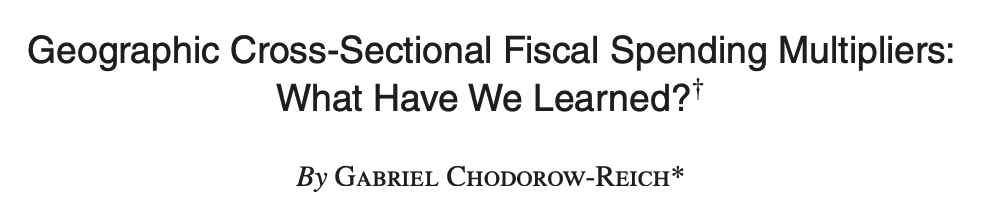
\includegraphics[width=\linewidth]{images/chodorowreich1.png}\\
      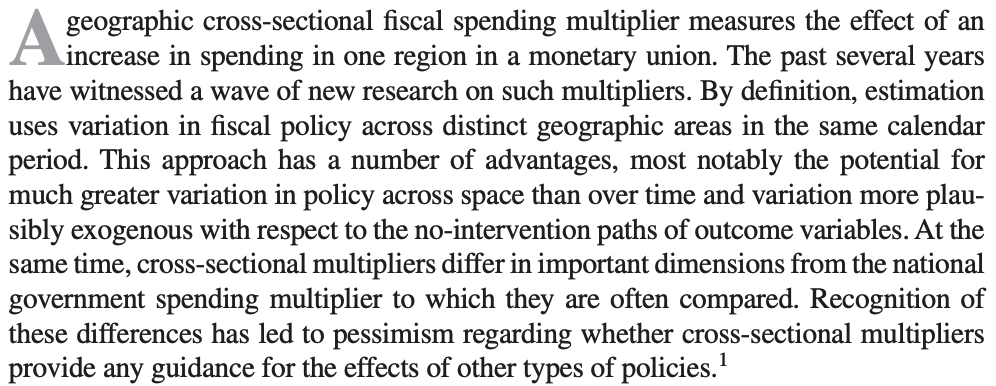
\includegraphics[width=\linewidth]{images/chodorowreich2.png}\\
      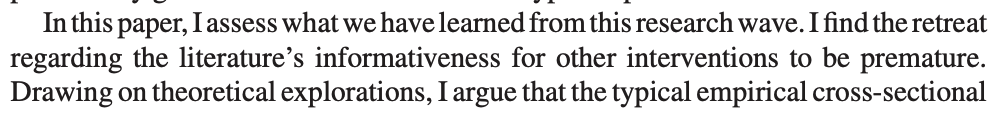
\includegraphics[width=\linewidth]{images/chodorowreich3.png}\\
            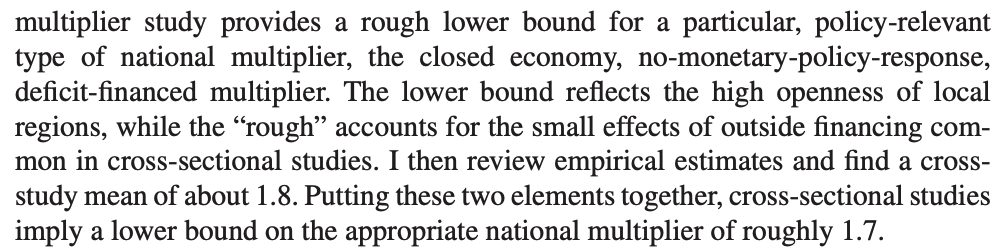
\includegraphics[width=\linewidth]{images/chodorowreich4.png}\\
    \end{center}
  \end{column}
\end{columns}
\end{frame}


\begin{frame}{Example 2: Sraer \& Thesmar (2020)}
\begin{columns}[T] % align columns
  \begin{column}{.5\textwidth}
    \begin{wideitemize}
    \item Use cross-firm experiment to influence the allocation of credit
    \item Some firms got lots more credit! Some did not
    \item How to aggregate up this affect? E.g. the policy effect is
      estimated by differencing the impact of the change on those who
      were more directly exposed vs. not -- however, this doesn't tell
      us about the aggregate impact on the economy
    \item The paper argues, using economic theory, that these issues can be safely ignored under certain assumptions
    \item Back to a version of SUTVA!
    \end{wideitemize}
  \end{column}%
  \hfill%
  \begin{column}{.5\textwidth}
    \begin{center}
      \only<1>{
        
\includegraphics[width=\linewidth]{images/sraer0.png}
        }
      \only<2>{
        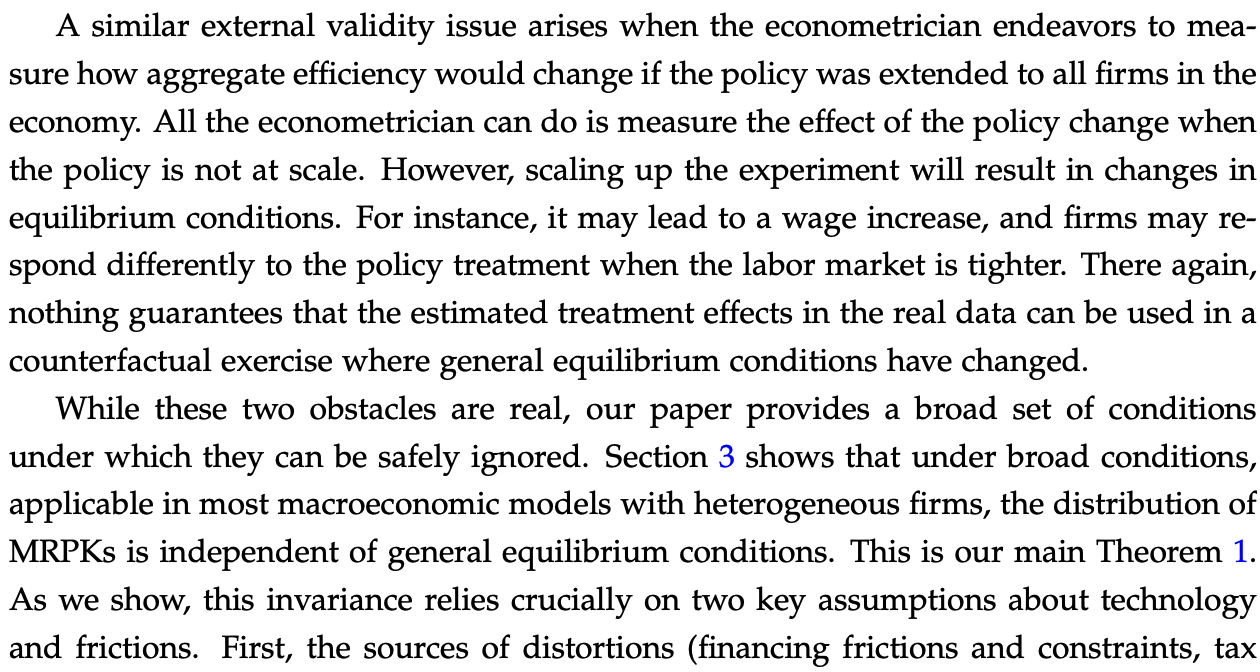
\includegraphics[width=\linewidth]{images/sraer1.png}
        }
    \end{center}
  \end{column}
\end{columns}

\end{frame}


\begin{frame}{Final thought: Dynamics}
\begin{columns}[T] % align columns
  \begin{column}{.5\textwidth}
    \begin{wideitemize}
    \item How to think about treatments staggered \emph{in time}? E.g. $\mathbf{Y}_{i} = (Y_{i1}, \ldots, Y_{iT})$
      \begin{itemize}
      \item What is the potential outcome? $Y_{it}(D_{it})$?  $Y_{it}(D_{it}, D_{it-1})$? 
      \end{itemize}
    \item We have a vector of outcomes over time -- what effects can we identify treatments on? What restrictions do we need to make?
    \item Consider the mRNA Covid Vaccine trials -- what assumptions do we need to identify the effect of just one dose?
    \end{wideitemize}
  \end{column}%
  \hfill%
  \begin{column}{.5\textwidth}
    \begin{center}
        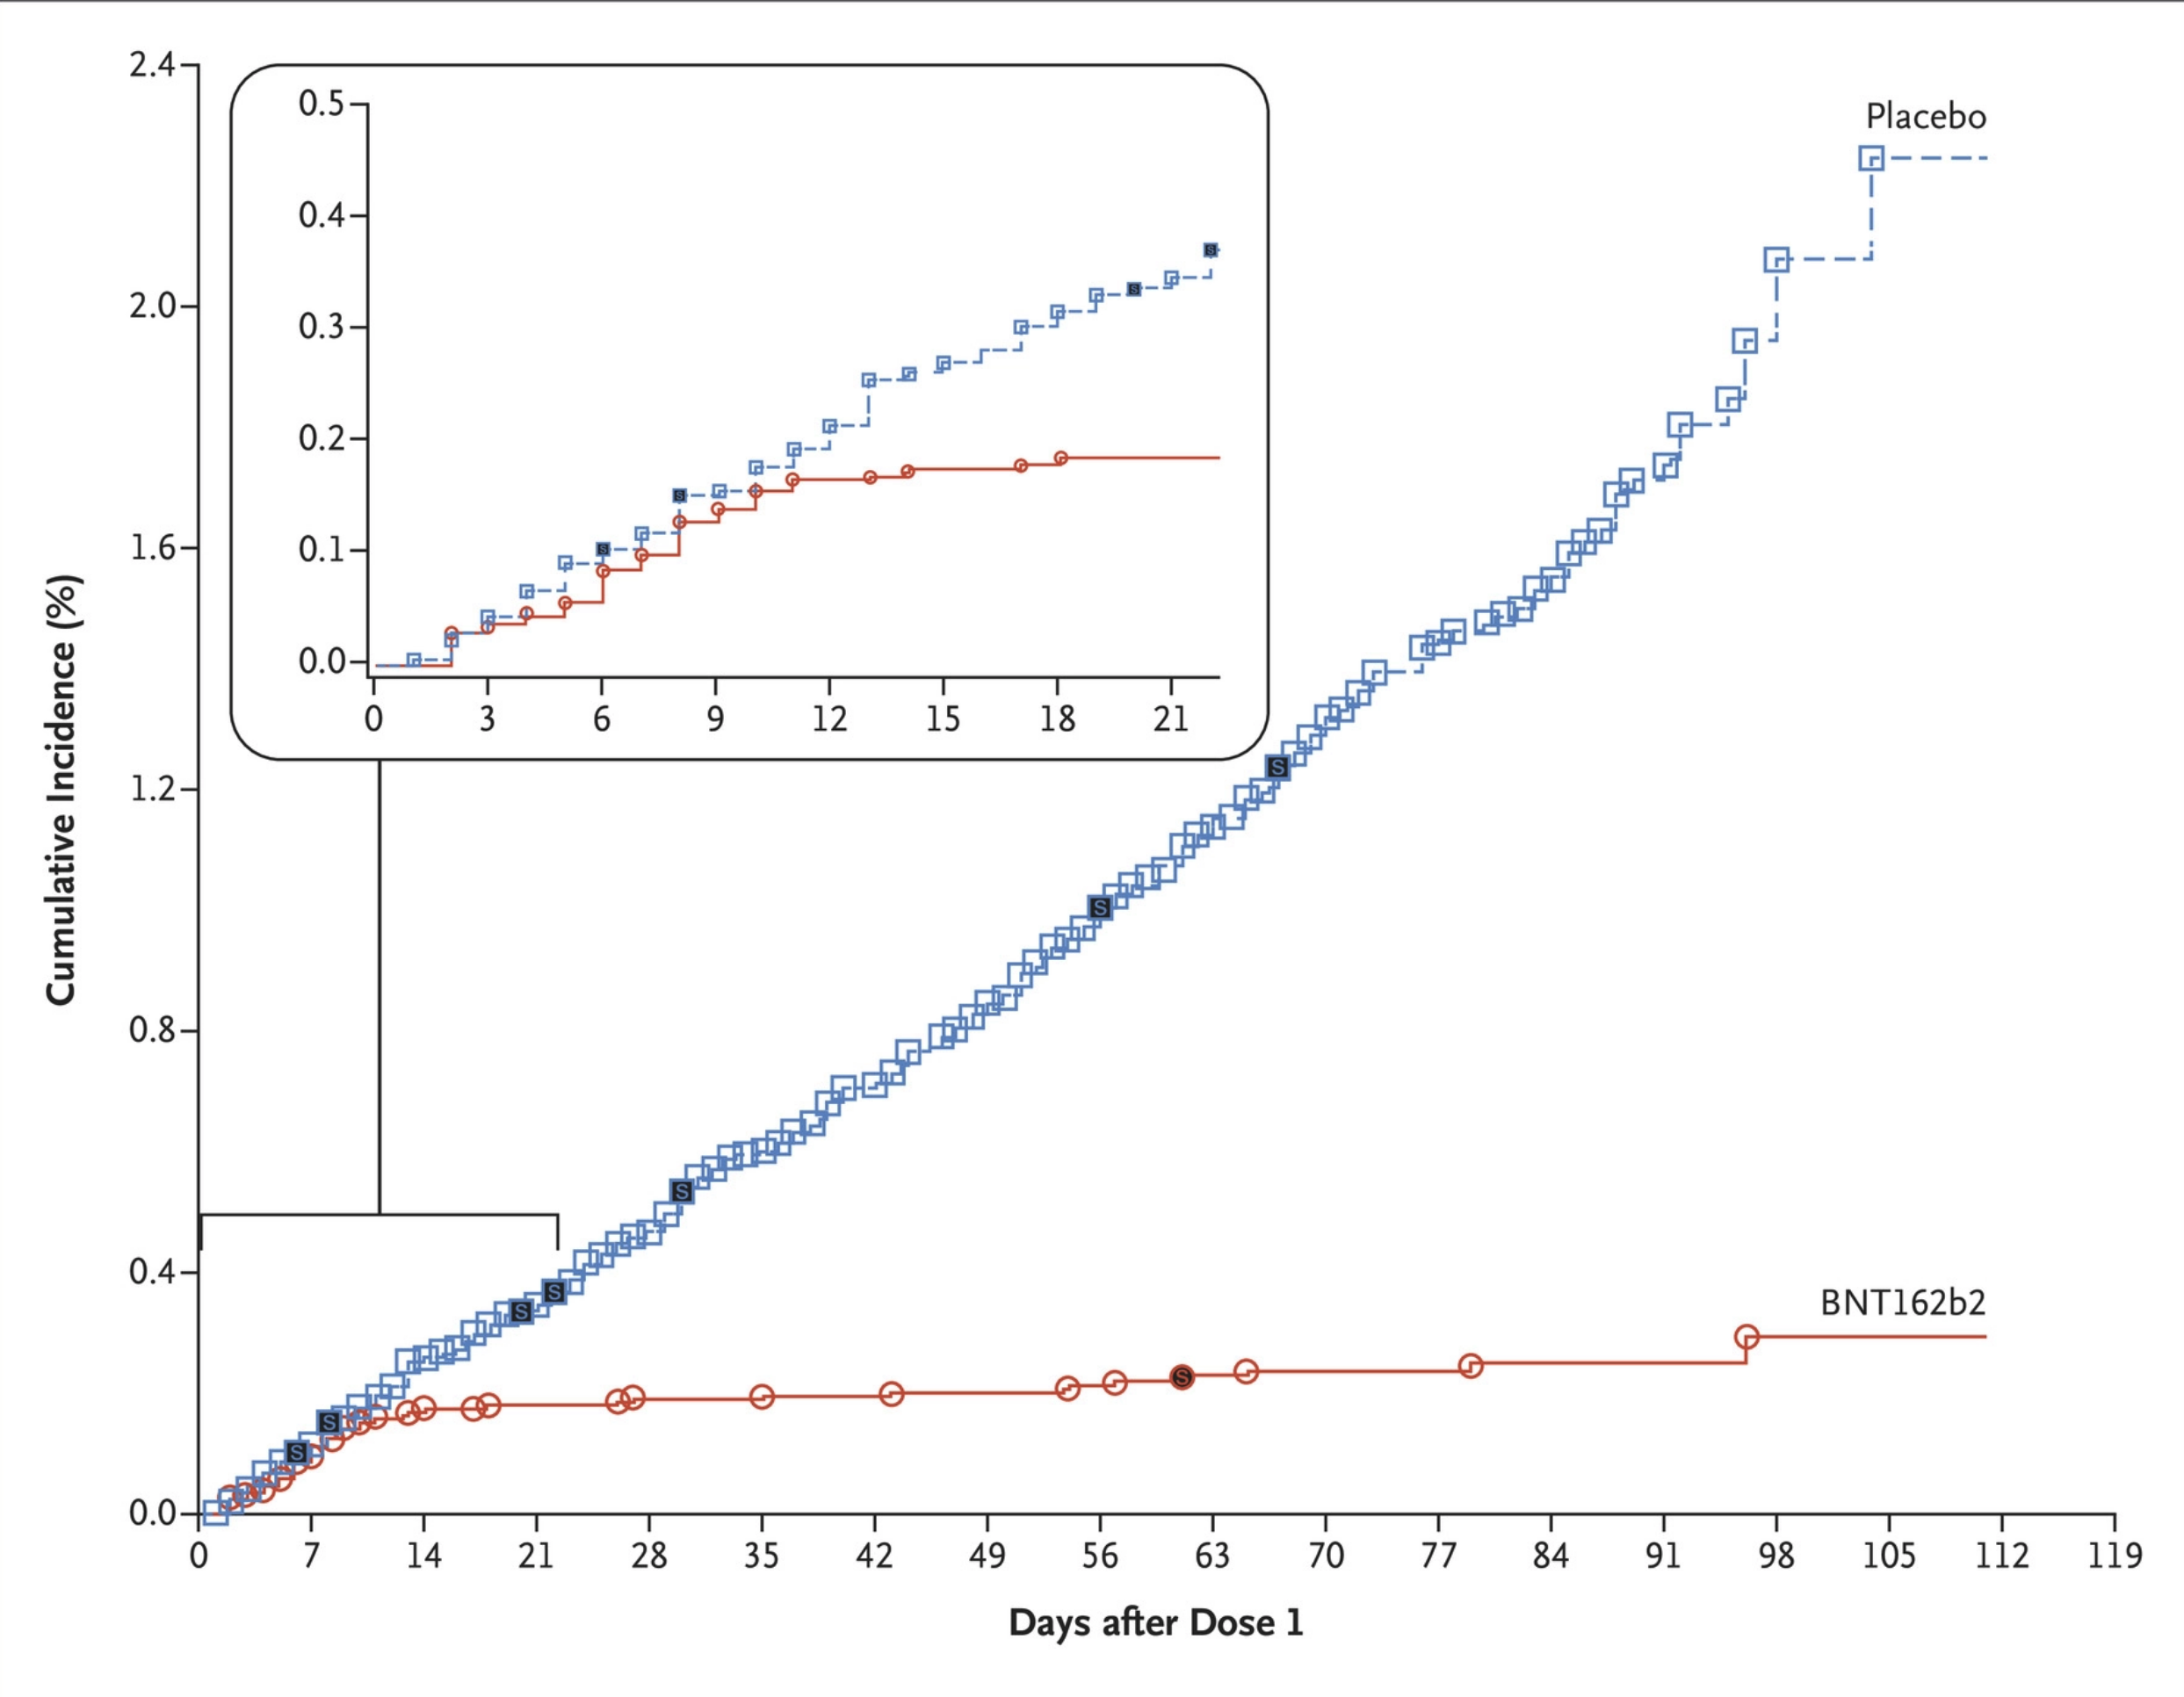
\includegraphics[width=\linewidth]{images/vaccine_dynamics.png}
    \end{center}
  \end{column}
\end{columns}

\end{frame}



\end{document}





\begin{columns}[T] % align columns
  \begin{column}{.5\textwidth}
  \end{column}%
  \hfill%
  \begin{column}{.5\textwidth}
    \begin{center}
    \end{center}
  \end{column}
\end{columns}

